%
% lemniskate.tex
%
% (c) 2021 Prof Dr Andreas Müller, OST Ostschweizer Fachhochschule
%
\section{Lemniskatischer Sinus
\label{buch:elliptisch:section:lemniskate}}
\rhead{Lemniskatischer Sinus}
Historisch war der {\em lemniskatische Sinus} die erste ellptische
Funktion, die Gauss bereits als 19-jähriger untersucht, aber nicht 
veröffentlich hat.
In diesem Abschnitt soll die Verbindung zu den Jacobischen
elliptischen Funktionen hergestellt werden.

\subsection{Lemniskate
\label{buch:gemotrie:subsection:lemniskate}}
\begin{figure}
\centering
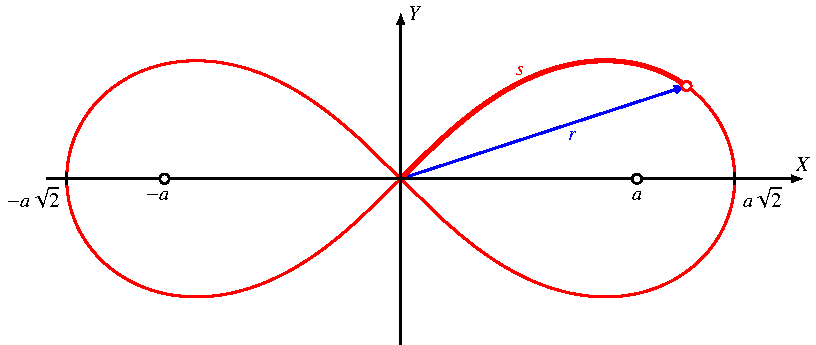
\includegraphics{chapters/110-elliptisch/images/lemniskate.pdf}
\caption{Bogenlänge und Radius der Lemniskate von Bernoulli.
\label{buch:elliptisch:fig:lemniskate}}
\end{figure}
Die Lemniskate von Bernoulli ist die Kurve vierten Grades mit der Gleichung
\begin{equation}
(x^2+y^2)^2 = 2a^2(x^2-y^2).
\label{buch:elliptisch:eqn:lemniskate}
\end{equation}
Sie ist in Abbildung~\ref{buch:elliptisch:fig:lemniskate}
dargestellt.
Die beiden Scheitel der Lemniskate befinden sich bei $x=\pm a/\sqrt{2}$.

In Polarkoordinaten $x=r\cos\varphi$ und $y=r\sin\varphi$
gilt nach Einsetzen in \eqref{buch:elliptisch:eqn:lemniskate}
\begin{equation}
r^4
=
2a^2r^2(\cos^2\varphi-\sin^2\varphi)
=
2a^2r^2\cos2\varphi
\qquad\Rightarrow\qquad
r^2 = 2a^2\cos 2\varphi
\label{buch:elliptisch:eqn:lemniskatepolar}
\end{equation}
als Darstellung der Lemniskate in Polardarstellung.
Sie gilt für Winkel $\varphi\in[-\frac{\pi}4,\frac{\pi}4]$ für das
rechte Blatt und $\varphi\in[\frac{3\pi}4,\frac{5\pi}4]$ für das linke
Blatt der Lemniskate.

Für die Definition des lemniskatischen Sinus wird eine Skalierung
verwendet, die den rechten Scheitel im Punkt $(1,0)$.
Dies ist der Fall für $a=1/\sqrt{2}$, die Gleichung der Lemniskate
wird dann zu
\[
(x^2+y^2)^2 = 2(x^2-y^2).
\]

\subsubsection{Bogelänge}
Die Funktionen
\begin{equation}
x(r) = \frac{r}{\sqrt{2}}\sqrt{1+r^2},
\quad
y(r) = \frac{r}{\sqrt{2}}\sqrt{1-r^2}
\label{buch:geometrie:eqn:lemniskateparam}
\end{equation}
erfüllen
\begin{align*}
x(r)^2-y(r)^2
&=
\frac{r^2(1+r^2)}{2}-\frac{r^2(1-r^2)}{2}
\\
&
=
r^4
=
(x(r)^2 + y(r)^2)^2,
\end{align*}
sie stellen also eine Parametrisierung der Lemniskate dar.

Mit Hilfe der Parametrsierung~\eqref{buch:geometrie:eqn:lemniskateparam}
kann man die Länge $s$ des in Abbildung~\ref{buch:elliptisch:fig:lemniskate}
dargestellten Bogens der Lemniskate berechnen.
Dazu benötigt man die Ableitungen nach $r$, die man mit der Produkt- und
Kettenregel berechnen kann:
\begin{align*}
\dot{x}(r)
&=
\frac{\sqrt{1+r^2}}{\sqrt{2}}
+
\frac{r^2}{\sqrt{2}\sqrt{1+r^2}}
&&\Rightarrow&
\dot{x}(r)^2
&=
\frac{1+r^2}{2} +r^2 + \frac{r^4}{2(1+r^2)}
\\
\dot{y}(r)
&=
\frac{\sqrt{1-r^2}}{\sqrt{2}}
-
\frac{r^2}{\sqrt{2}\sqrt{1-r^2}}
&&\Rightarrow&
\dot{y}(r)^2
&=
\frac{1-r^2}{2} -r^2 + \frac{r^4}{2(1-r^2)}
\end{align*}
Die Summe der Quadrate ist
\begin{align*}
\dot{x}(r)^2 + \dot{y}(r)^2
&=
1 + r^4\frac{1-r^2+1+r^2}{2(1+r^2)(1-r^2)}
=
1+r^4\frac{2}{2(1-r^4)}
=
\frac{1-r^4+r^4}{1-r^4}
=
\frac1{1-r^4}.
\end{align*}
Durch Einsetzen in das Integral für die Bogenlänge bekommt man
\begin{equation}
s(r)
=
\int_0^r
\frac{1}{\sqrt{1-t^4}}\,dt.
\label{buch:elliptisch:eqn:lemniskatebogenlaenge}
\end{equation}

\subsubsection{Darstellung als elliptisches Integral}
Das unvollständige elliptische Integral erster Art mit Parameter
$m=-1$ ist
\[
F(r,-1)
=
\int_0^x \frac{dt}{\sqrt{(1-t^2)(1-(-1)t^2)}}
=
\int_0^x \frac{dt}{\sqrt{1-t^4}}
=
s(r).
\]
Der lemniskatische Sinus ist also eine Umkehrfunktion des
ellptischen Integrals erster Art für einen speziellen Wert des
Parameters $m$

\subsubsection{Der lemniskatische Sinus und Kosinus}
Berechnet die Gegenkathete zu einer gegebenen Bogenlänge des Kreises.
Daher ist es naheliegend, die Umkehrfunktion von $s(r)$ in 
\eqref{buch:elliptisch:eqn:lemniskatebogenlaenge}
den {\em lemniskatischen Sinus} zu nennen mit der Bezeichnung
$r=\operatorname{sl} s$.

Der Kosinus ist der Sinus des komplementären Winkels.
Auch für die lemniskatische Bogenlänge $s(r)$ lässt sich eine
komplementäre Bogenlänge definieren, nämlich die Bogenlänge zwischen
dem Punkt $(x(r), y(r))$ und $(1,0)$.
Die Länge des rechten Blattes der Lemniskate wird mit $\varpi$ bezeichnet
und hat den numerischen Wert
\[
\varphi
=
2\int_0^1\sqrt{\frac{1}{1-t^4}}\,dt
=
2.6220575542.
\]
Lemniskatenbogens zwischen dem Nullpunkt und $(1,0)$ hat die Länge
$\varpi/2$.

Der {\em lemniskatische Kosinus} von $s$ ist derjenige Radiuswert $r$,
für den der Lemniskatenbogen zwischen $(x(r), y(r))$ und $(1,0)$
die Länge $s$ hat.


XXX Algebraische Beziehungen \\
XXX Ableitungen \\
